%-----------------------------------------------------------------------------%
\chapter{\babEmpat}
%-----------------------------------------------------------------------------%
Selama pelaksanaan Kerja Praktik di BMW Laboratory, NTUST, penulis terlibat dalam beberapa proyek utama dan kegiatan pendukung yang berfokus pada pengembangan ``Wifi RAN Digital Twin'' dan teknologi terkait. Bab ini akan merinci pelaksanaan kegiatan-kegiatan tersebut.

%-----------------------------------------------------------------------------%
\section{Masa Percobaan dan Pembelajaran Awal}
%-----------------------------------------------------------------------------%
Periode awal kerja praktik (4 April 2025 sampai 25 Juni 2025) difokuskan pada pembelajaran ilmu fondasi dan pengembangan kemampuan dasar yang menjadi landasan untuk proyek-proyek selanjutnya. Kegiatan pada masa ini dibagi menjadi dua area utama: pembelajaran ilmu dasar dan pengembangan awal pengumpul data.

Seluruh kegiatan pada masa percobaan didokumentasikan dengan membuat \textit{study notes} dalam format Markdown, yang kemudian diunggah ke repositori GitHub BMW Lab. Dokumentasi ini mencakup hal-hal yang penting untuk referensi di masa depan, termasuk kode contoh, diagram, poin-poin penting, dan tautan ke sumber daya eksternal.

\subsection{Pembelajaran Ilmu Dasar}

Pada tahap awal, penulis mempelajari konsep-konsep dasar yang relevan dengan proyek, termasuk arsitektur 5G, standar O-RAN, dan konsep Wifi. Studi tentang arsitektur 5G mencakup pemahaman tentang jaringan inti 5G, teknologi radio akses, dan kasus penggunaan utama 5G seperti eMBB, URLLC, dan mMTC. Penulis juga mempelajari mempelajari standar O-RAN, dengan fokus pada Spesifikasi Antarmuka O1 yang menjadi dasar pengembangan \textit{WiFi Adapter}. Selain itu, penulis mempelajari konsep dasar WiFi, termasuk arsitektur jaringan WiFi, frekuensi dan channel WiFi, serta metrik kinerja seperti RSSI dan SNR

Secara keseluruhan, terdapat 9 dokumen \textit{study notes} yang dibuat selama periode ini, mencakup topik-topik berikut:

\begin{enumerate}
    \item TEEP Intern Administration: Dokumen ini mencakup informasi administratif terkait kerja praktik, termasuk panduan panduan umum dan prosedur laboratorium
    \item Foundation: Dokumen ini merangkum konsep-konsep soft skill yang diberi sebelum memulai kerja praktik, seperti manajemen waktu, komunikasi efektif, dan kolaborasi tim.
    \item Gitlab: Dokumen ini merangkum perbandingan antara GitLab dan GitHub untuk digunakan dalam manajemen proyek-proyek di laboratorium.
    \item O-RAN: Dokumen ini merangkum konsep dasar Open Radio Access Network (O-RAN), termasuk arsitektur, antarmuka, dan standar yang relevan.
    \item OAI: Dokumen ini merangkum konsep dasar OpenAirInterface (OAI), sebuah implementasi open-source dari jaringan 5G.
    \item Infrastructure: Dokumen ini merangkum arsitektur infrastruktur laboratorium, khususnya yang berkaitan dengan server.
    \item Playwright: Dokumen ini merangkum penggunaan Playwright untuk web scraping, yang menjadi dasar pengembangan pengumpul data awal.
    \item WiFI Basics: Dokumen ini merangkum konsep dasar WiFi serta hubungan dengan 5G dan O-RAN.
    \item O1 Interface: Dokumen ini merangkum spesifikasi antarmuka O1 dari O-RAN, yang menjadi dasar pengembangan \textit{WiFi Adapter}, khususnya pada aspek Virtualized Evolved Services (VES) untuk Performance Management (PM).
\end{enumerate}

Selain pada masa percobaan, penulis juga terus memperbarui dokumen-dokumen ini selama pelaksanaan kerja praktik luring. Dokumen-dokumen yang telah dibuat pada masa luring meliputi:

\begin{enumerate}
    \item TEIV: Dokumen ini merangkum konsep dasar Topology Exposure \& Inventory Common (TEIV) yang diperlukan untuk melakukan \textit{code review}.
    \item NS3: Dokumen ini merangkum konsep dasar Network Simulator 3 (NS-3) yang diperlukan untuk memahami simulasi jaringan.
    \item Sionna: Dokumen ini merangkum konsep dasar NVIDIA Sionna, sebuah simulator jaringan yang dapat memodelkan propagasi signal.
    \item Electromagnetic: Dokumen ini merangkum konsep dasar elektromagnetik yang relevan untuk memahami propagasi sinyal WiFi.
    \item Antenna and Propagation: Dokumen ini merupakan lanjutan dari dokumen elektromagnetik, dengan fokus pada konsep antena dan propagasi sinyal.
    \item External Influx: Dokumen ini merangkum cara menghubungkan InfluxDB eksternal pada SMO.
    \item Gradient Descent: Dokumen ini merangkum konsep dasar algoritma optimisasi
\end{enumerate}
	
\subsection{Pengembangan Awal Pengumpul Data}
Sebagai langkah awal untuk pengumpulan data, penulis meneliti berbagai metode untuk mengekstrak data dari perangkat jaringan Unifi. Metode \textit{web scraping} dipilih sebagai pendekatan awal. Penulis mempelajari pustaka Playwright dan berhasil mengembangkan skrip untuk secara otomatis masuk ke dasbor Unifi, menavigasi antarmuka, dan mengumpulkan data metrik dari \textit{Access Point} (AP). Skrip ini menjadi poin awal dari penulis menggunakan dan mengembangkan \textit{WiFi Adapter} yang digunakan di laboratorium.

\begin{figure}[htbp]
    \centering
    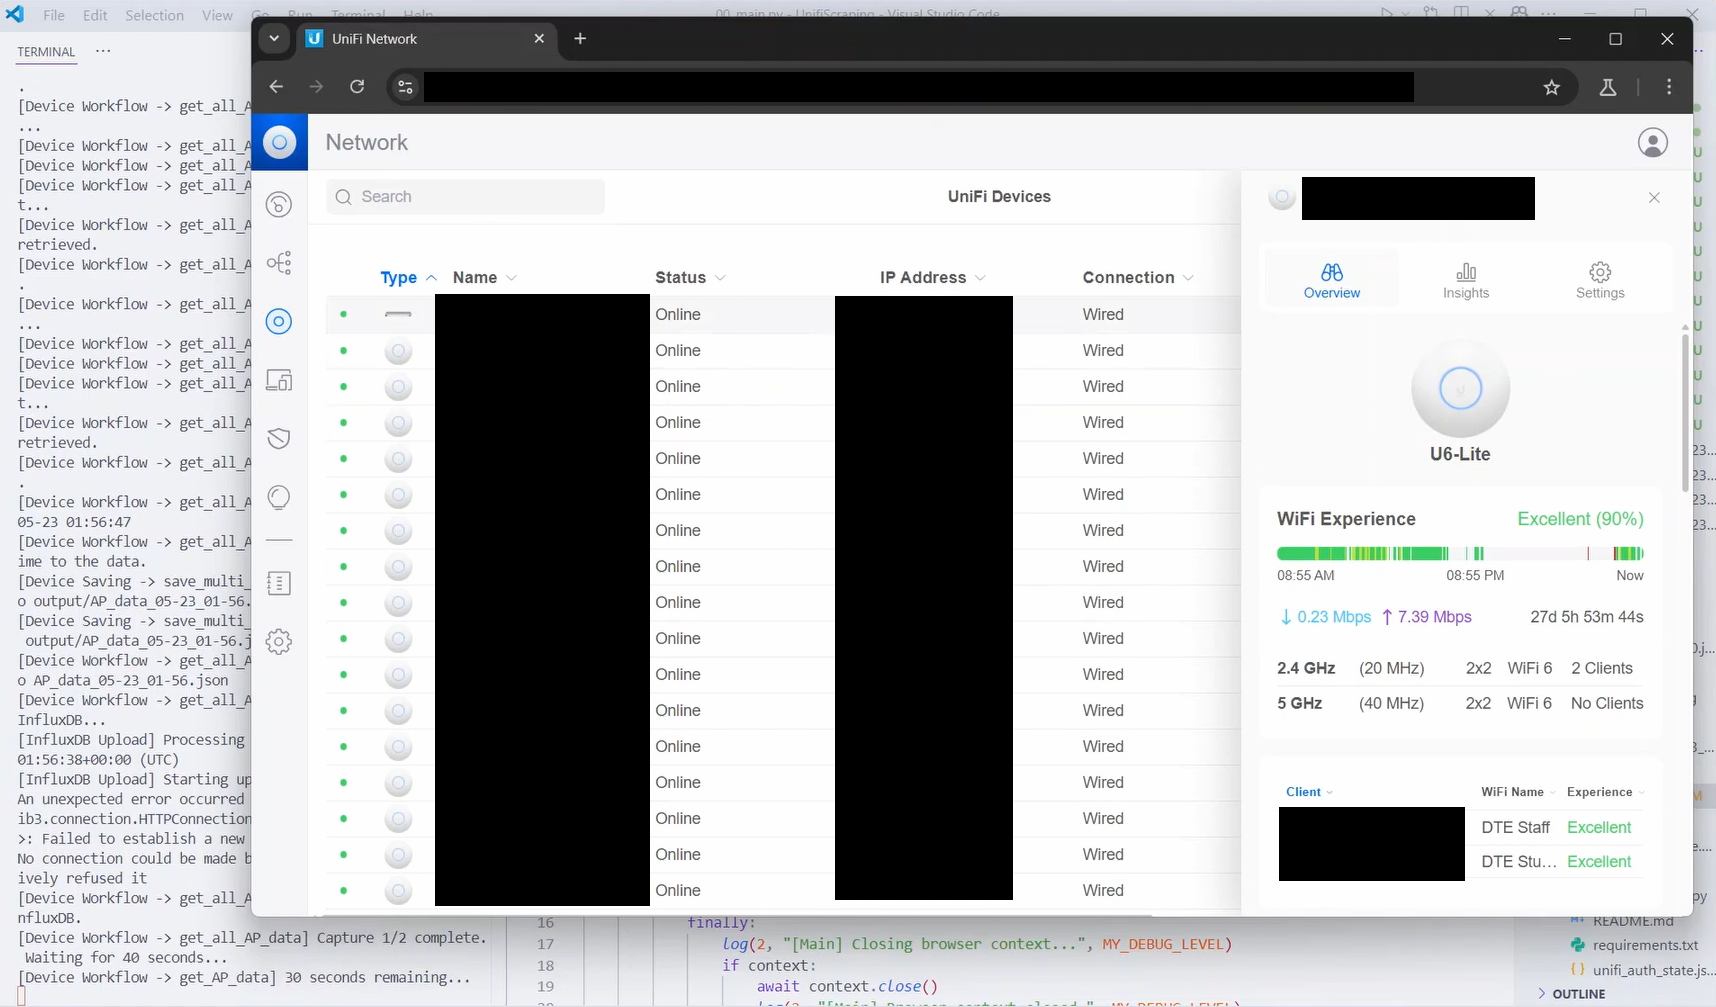
\includegraphics[width=0.8\textwidth]{assets/pics/unifi.png}
    \caption{Proses web scraping pada dasbor Ubiquiti Unifi, disensorkan untuk keamanan}
    \label{fig:unifi}
\end{figure}

Pengembangan skrip ini menggunakan struktur kode modular dan mengikuti format yang akan digunakan dalam \textit{WiFi Adapter} laboratorium. Dengan demikian, penulis dapat dengan mudah memahami alur kode WiFi Adapter dan dapat mudah mengembangkannya lebih lanjut di masa depan.

Skrip menggunakan metode \textit{web scraping} dengan Playwright; saat program dijalankan, skrip akan membuka browser secara otomatis, masuk ke dasbor Unifi menggunakan kredensial yang disediakan, menavigasi ke halaman yang berisi metrik AP, dan mengekstrak data yang diperlukan untuk setiap AP (dapat dilihat pada gambar \ref{fig:unifi}). Data yang dikumpulkan meliputi Nama AP, jumlah klien terhubung, dan statistik lalu lintas. Data ini kemudian diformat dan disimpan dalam file JSON (seperti yang ditunjukkan pada gambar \ref{fig:unifijson}).

\begin{figure}[htbp]
    \centering
    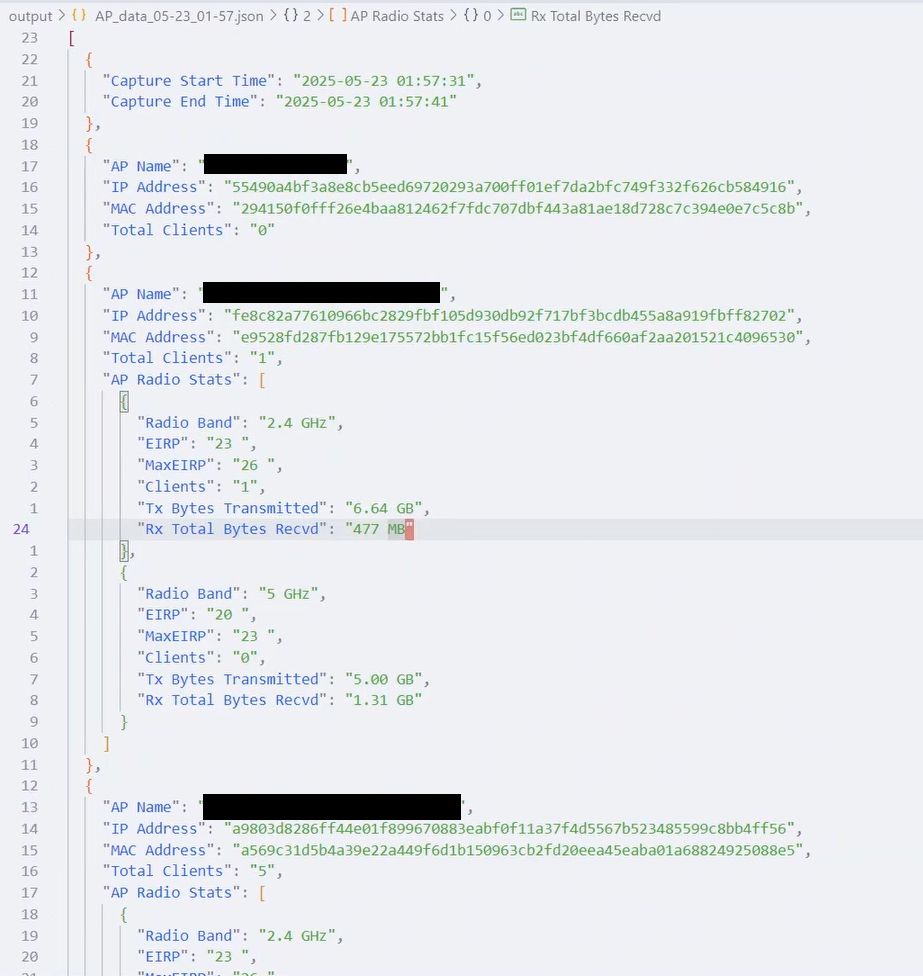
\includegraphics[width=0.5\textwidth]{assets/pics/unifijson.png}
    \caption{Data JSON yang dihasilkan dari proses web scraping, disensorkan untuk keamanan}
    \label{fig:unifijson}
\end{figure}


%-----------------------------------------------------------------------------%

\section{Proyek 1: WiFi Adapter untuk Integrasi O-RAN}
%-----------------------------------------------------------------------------%
Proyek ini bertujuan untuk membuat komponen perangkat lunak yang dapat mengumpulkan data dari infrastruktur WiFi di dunia nyata dan memformatnya agar sesuai dengan spesifikasi antarmuka O-RAN O1 untuk sistem \textit{Service Management and Orchestration} (SMO).

\subsection{Arsitektur dan Alur Kerja Data}
Jembatan antara WiFi RAN dan O-RAN SMO diimplementasikan sebagai WiFi O1 Node. Komponen ini terdiri dari dua bagian utama: O1 Agent yang mengekspos antarmuka NETCONF ke SMO, dan O1 Adapter yang bertugas mengambil dan memproses data dari vendor WiFi. Kontribusi utama dalam proyek ini berfokus pada pengembangan kedua komponen tersebut.

\begin{figure}[htbp]
    \centering
    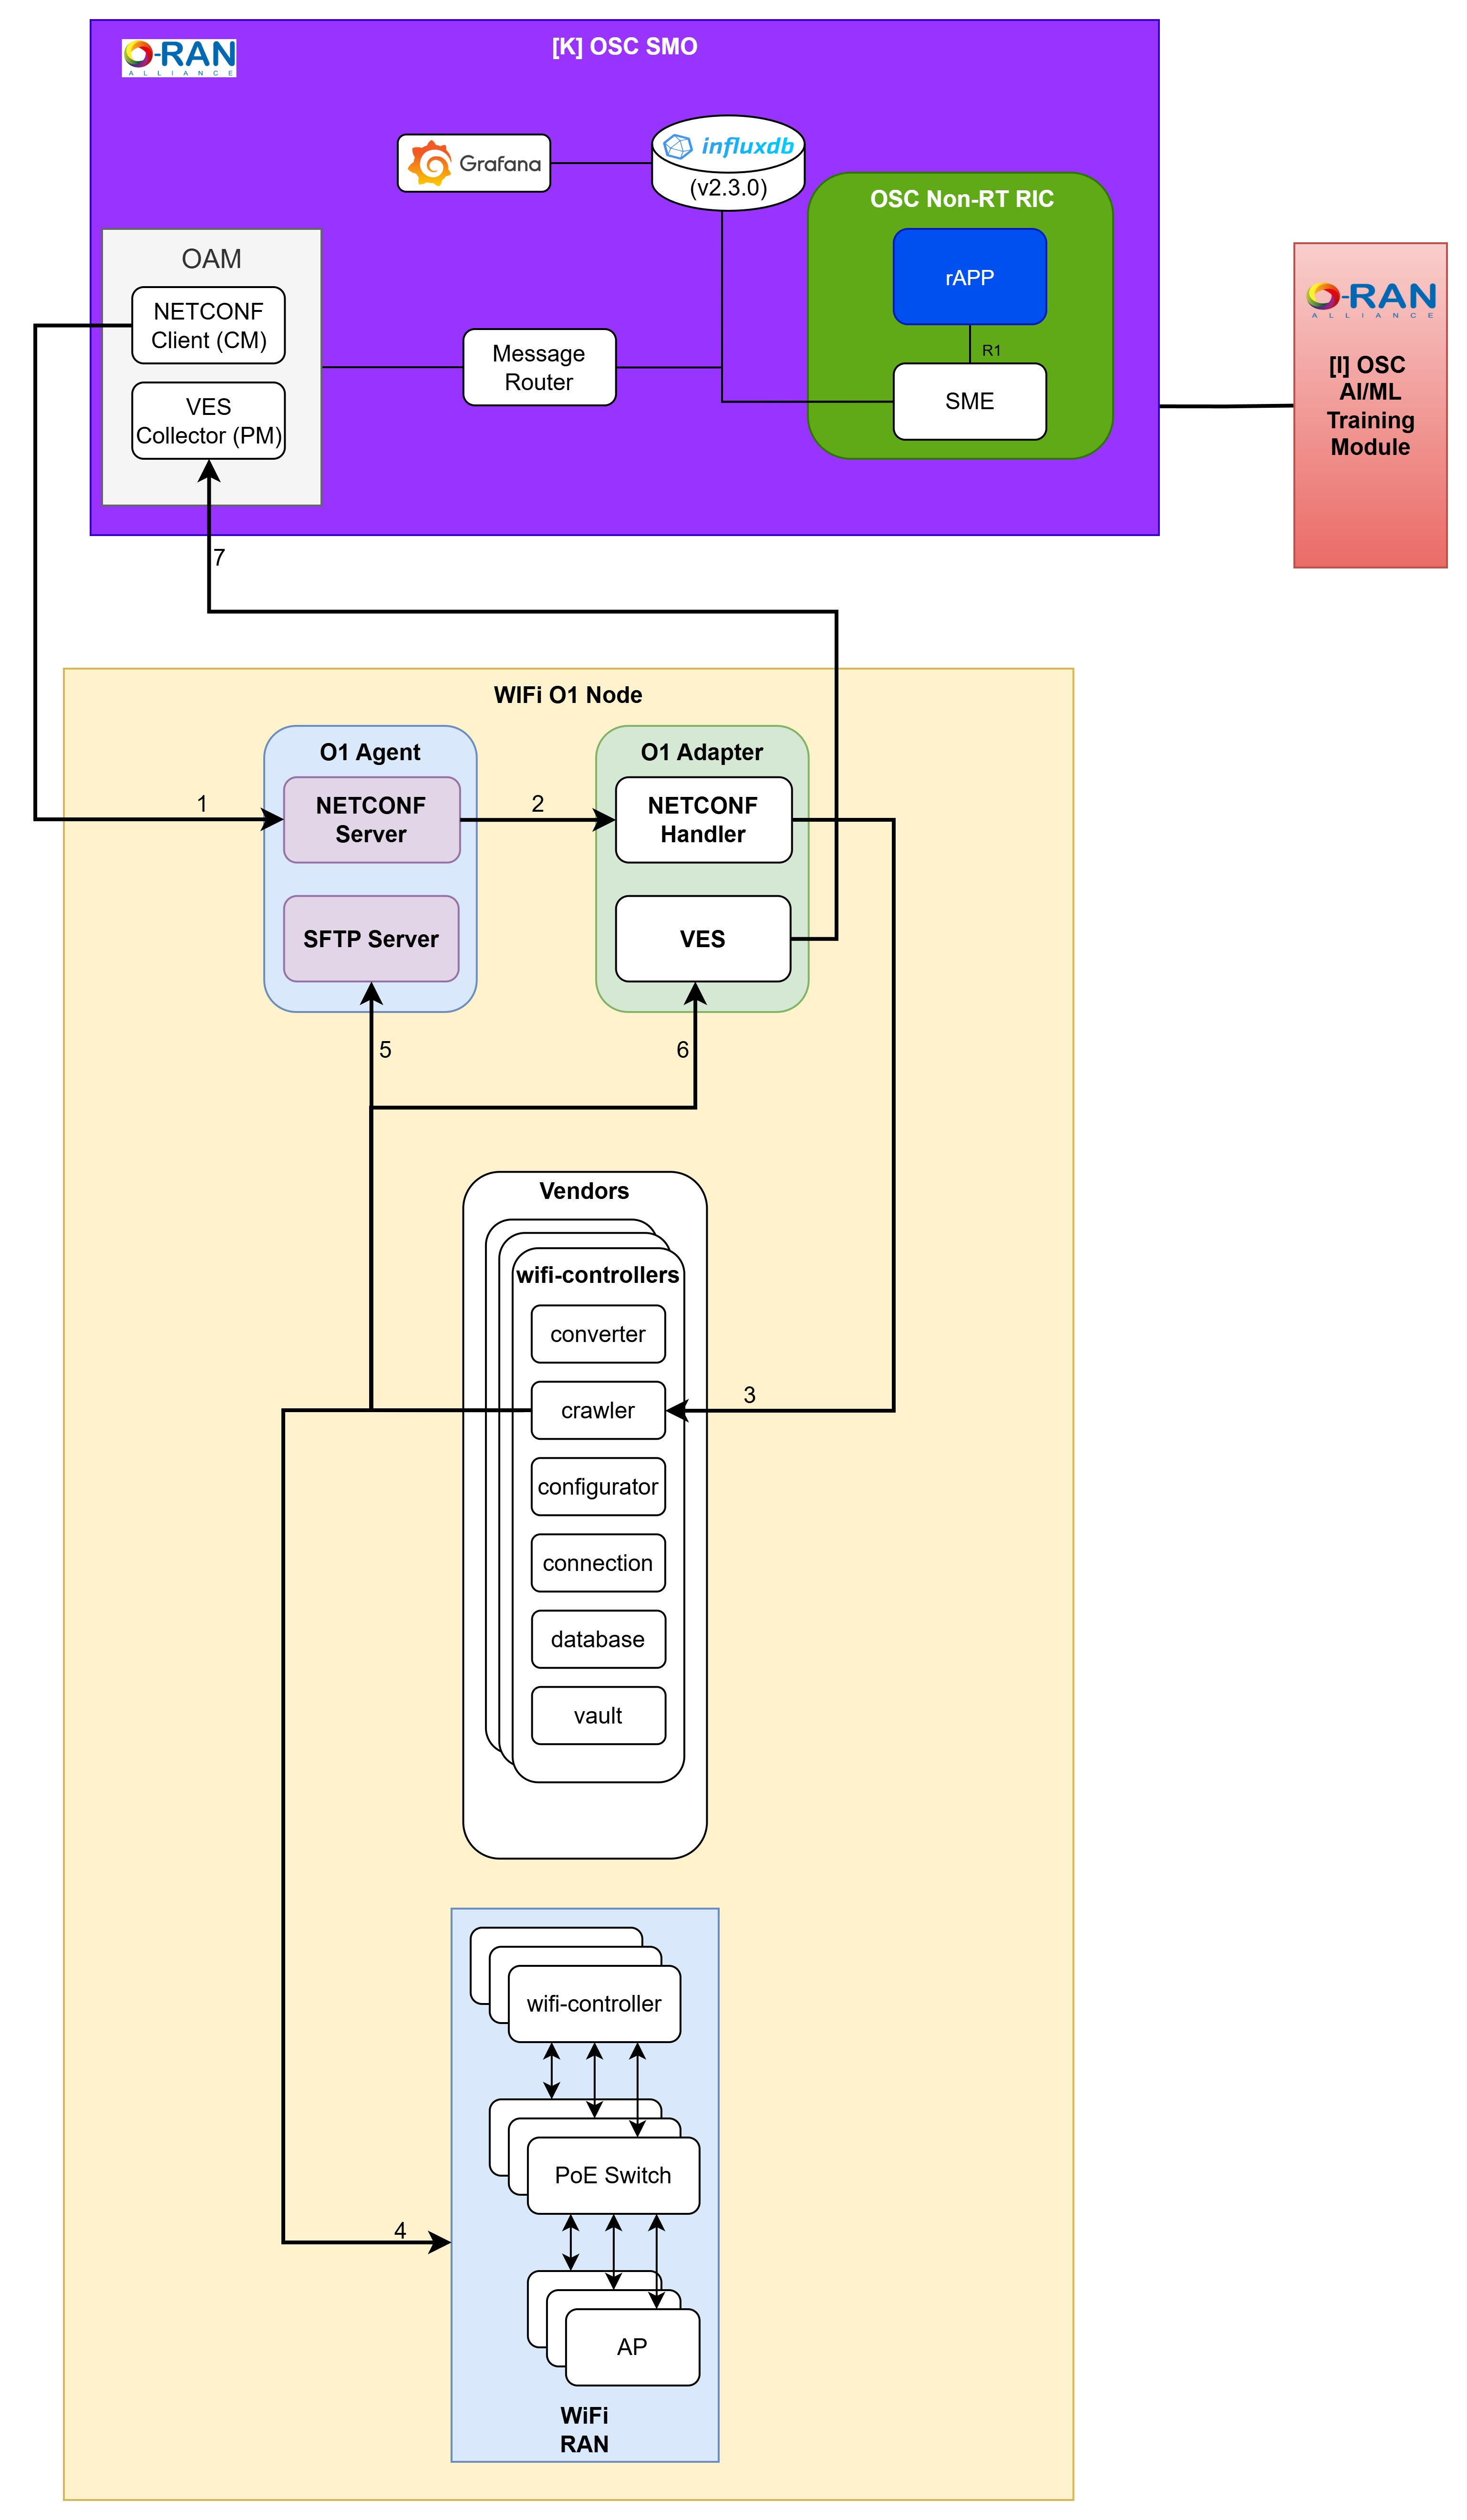
\includegraphics[width=0.8\textwidth]{assets/pics/smo_architecture.jpg}
    \caption{Arsitektur Integrasi WiFi RAN dengan O-RAN SMO}
    \label{fig:smo_architecture}
\end{figure}

Arsitektur adapter dirancang secara modular untuk mendukung berbagai vendor, dengan fokus awal pada Aruba dan HPE. Adapter ini terdiri dari beberapa layanan mikro:
\begin{itemize}
    \item \textbf{Connection}: Mengelola koneksi ke perangkat (misalnya, WiFi controller).
    \item \textbf{Crawler}: Mengambil data mentah dari perangkat.
    \item \textbf{Converter}: Mengubah data mentah menjadi format standar.
    \item \textbf{Vault}: Mengelola kredensial perangkat dengan aman.
    \item \textbf{Database}: Menyimpan data yang telah di-crawl (misalnya, di InfluxDB).
\end{itemize}

%-----------------------------------------------------------------------------%
\subsubsection{Alur Kerja Crawling NETCONF}
Proses pengumpulan data tidak berjalan terus-menerus, melainkan diinisiasi oleh SMO melalui antarmuka NETCONF.
\begin{enumerate}
    \item Inisiasi Pekerjaan (Job Initiation): SMO mengirimkan permintaan melalui NETCONF 3GPP PM Job Manager API, sebuah REST API untuk mengelola tugas \textit{Performance Measurement} (PM).
    \item Pembuatan Pekerjaan (Job Creation): Permintaan POST dikirim ke endpoint /managed-elements/\{me\_id\}/jobs dengan \textit{payload} JSON yang mendefinisikan pekerjaan. \textit{Payload} ini menentukan tipe data yang akan di-\textit{crawl} (misalnya, "job": "utilization") dan frekuensi pengumpulan (misalnya, "granularity": 30 detik). Pada gambar \ref{fig:netconf_api} dan gambar \ref{fig:json_payload} ditunjukkan contoh API dan \textit{payload} JSON untuk membuat pekerjaan PM.

\begin{figure}[htbp]
    \centering
    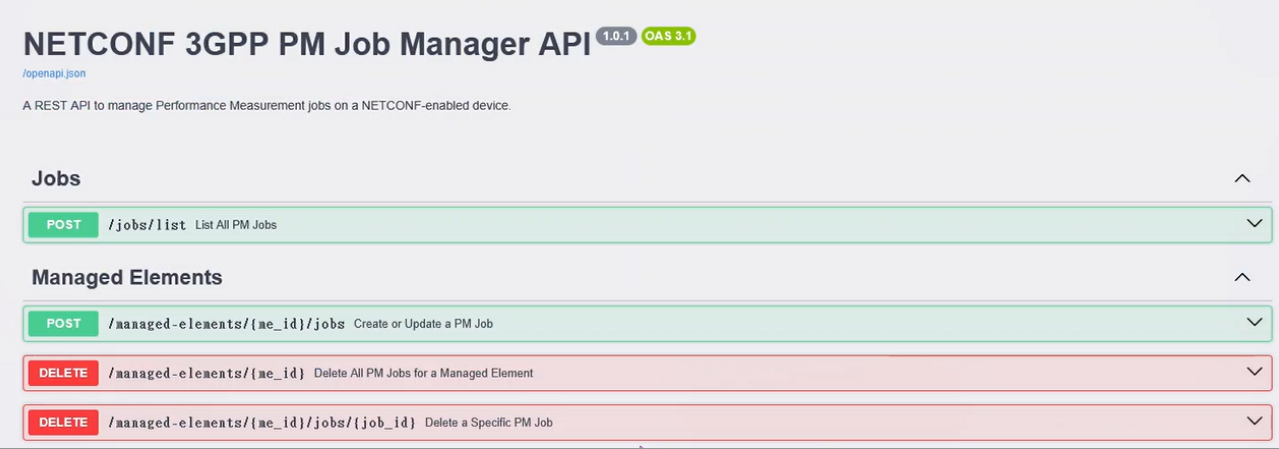
\includegraphics[width=0.8\textwidth]{assets/pics/netconf_api.png}
    \caption{NETCONF 3GPP PM Job Manager API}
    \label{fig:netconf_api}
\end{figure}

\begin{figure}[htbp]
    \centering
    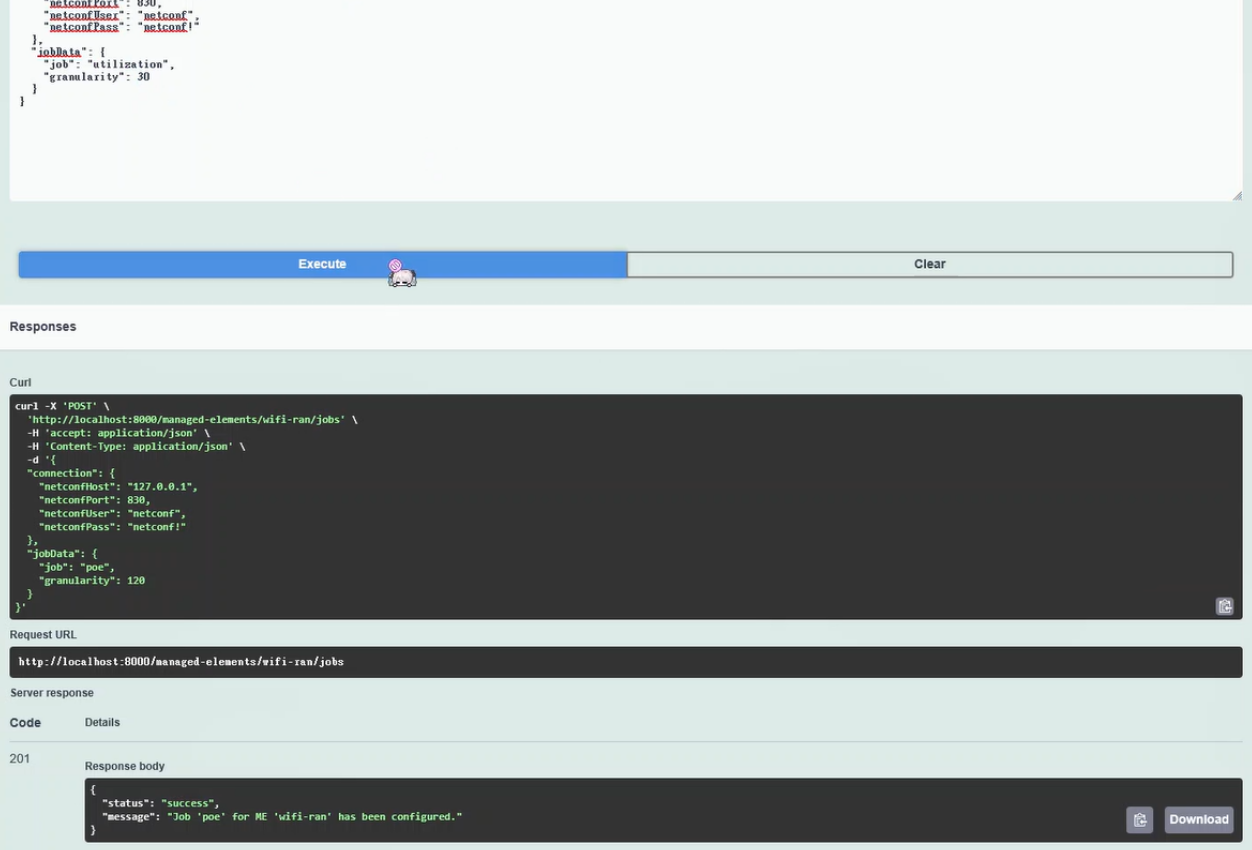
\includegraphics[width=0.8\textwidth]{assets/pics/json_payload.png}
    \caption{Contoh payload JSON untuk membuat PM job}
    \label{fig:json_payload}
\end{figure}

    \item Eksekusi dan Penyimpanan Data: Setelah pekerjaan dikonfigurasi, \textit{crawler} yang sesuai akan dieksekusi sesuai dengan granularitas yang ditentukan. Data yang berhasil di-crawl kemudian dikonversi ke format standar berbasis XML dan disimpan di SFTP Server.
    \item Setelah data disimpan, WiFi Adapter mengirimkan \textit{event} VES (Virtual Event Streaming) ke kolektor SMO untuk memberitahukan bahwa data baru tersedia.
    \item SMO kemudian mengambil file laporan PM dalam format XML dari SFTP Server dengan protokol SFTP dan menyimpannya di dalam \textit{database} InfluxDB internalnya.
\end{enumerate}

\begin{figure}[htbp]
    \centering
    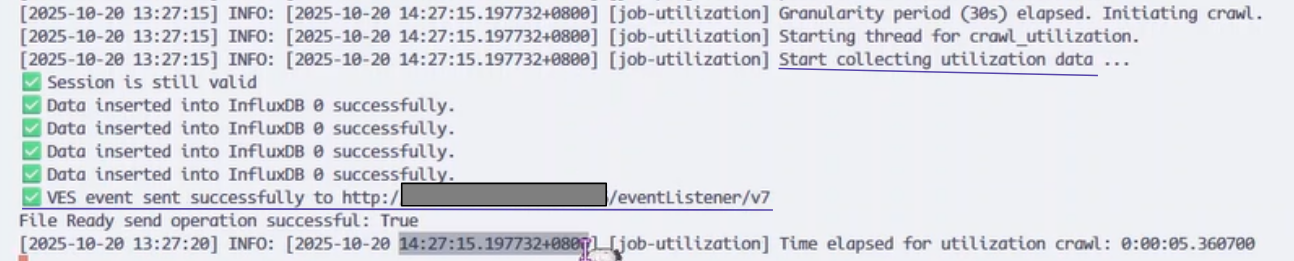
\includegraphics[width=0.8\textwidth]{assets/pics/crawler_log.png}
    \caption{Log crawler dan output server SFTP}
    \label{fig:crawler_log}
\end{figure}

Gambar \ref{fig:crawler_log} menunjukkan contoh log dari WiFi Adapter saat melakukan \textit{crawling} data dari utilizaation AP Aruba dan mengirimkan VES event ke SMO.

% %-----------------------------------------------------------------------------%
\subsubsection{Standardisasi Parameter dan Konversi XML}

Salah satu tantangan utama adalah standardisasi parameter, yaitu memetakan metrik spesifik vendor WiFi ke standar yang ditentukan oleh 3GPP dan O-RAN.

\begin{itemize}
    \item STA (Klien): Parameter Aruba seperti ``STA RSSI'' dipetakan ke standar O-RAN \texttt{OR.ULSQL.PuschRssi.SSB.statistic}.
    \item AP (Access Point): Parameter Aruba seperti ``Clients'' dipetakan ke standar 3GPP \texttt{RRC.ConnMean}, dan ``AP Tx Bytes'' dipetakan ke O-RAN \texttt{OR.PDCPB.UlPdcpSduDataVol}.
\end{itemize}

\begin{figure}[htbp]
    \centering
    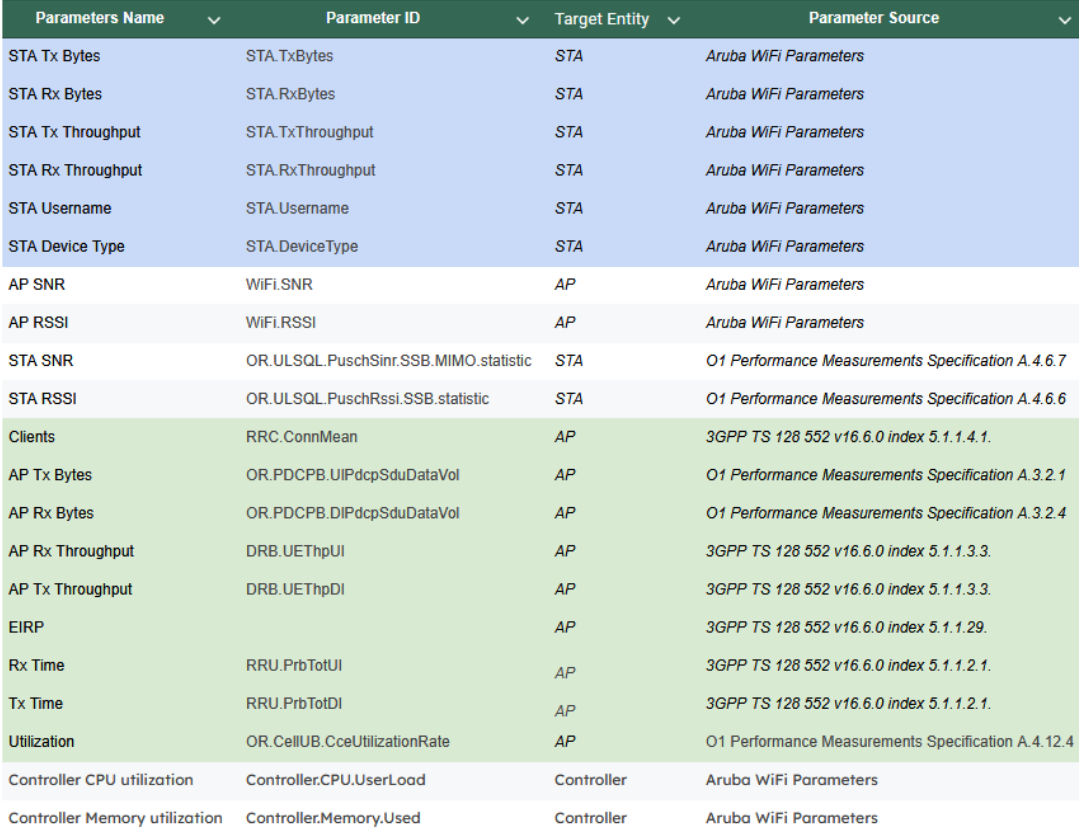
\includegraphics[width=0.8\textwidth]{assets/pics/param_standardization.png}
    \caption{Tabel Standardisasi Parameter}
    \label{fig:param_standardization}
\end{figure}

Pada gambar \ref{fig:param_standardization} ditunjukkan contoh tabel yang digunakan untuk memetakan parameter vendor ke standar O-RAN/3GPP. Jika metric didefinisikan pada kedua standar, maka prioritas diberikan pada standar 3GPP.

Data yang telah distandarisasi ini kemudian dikonversi dari format JSON internal ke format XML standar PM. Skrip Python digunakan untuk menghasilkan file XML yang mematuhi skema 3GPP \texttt{measCollecFile} (spesifikasi 32.435). File XML ini berisi data PM untuk beberapa AP, lengkap dengan \textit{timestamp} dan nilai metrik yang dipetakan ke \textit{measType} standar.

\begin{figure}[htbp]
    \centering
    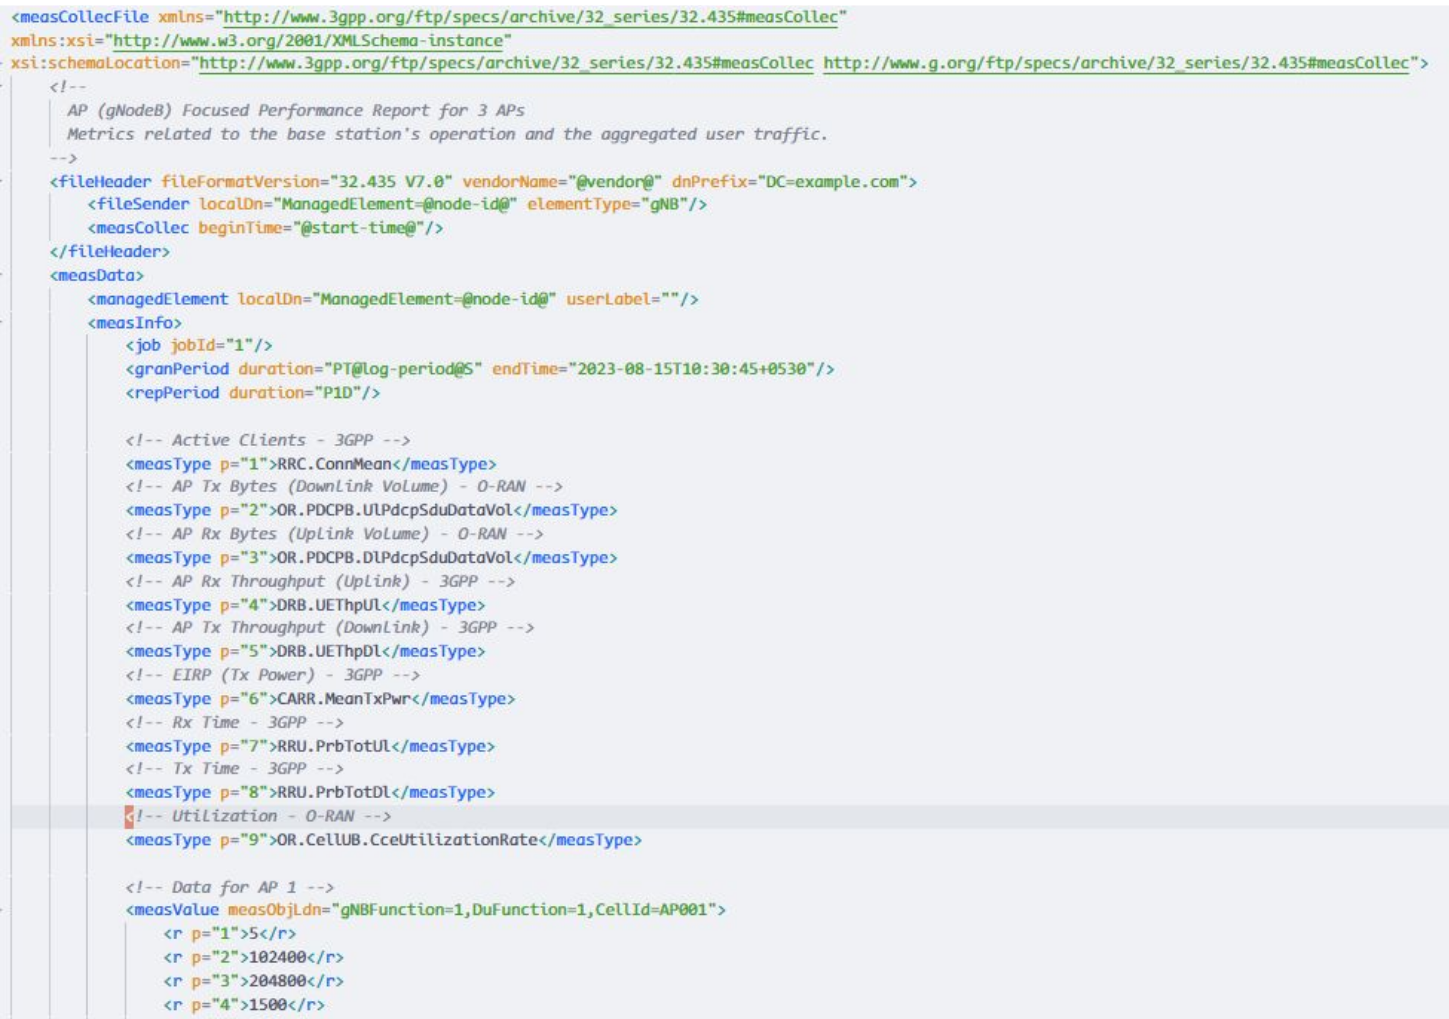
\includegraphics[width=0.8\textwidth]{assets/pics/xml_template.png}
    \caption{Contoh XML data PM}
    \label{fig:xml_template}
\end{figure}

Pada gambar \ref{fig:xml_template} ditunjukkan contoh XML AP yang dihasilkan, yang berisi data PM untuk beberapa AP dengan metrik yang telah distandarisasi. File XML ini kemudian diunggah ke SFTP Server untuk diambil oleh SMO.

%-----------------------------------------------------------------------------%
\subsection{Inisialisasi Crawler dan Integrasi SMO}
%-----------------------------------------------------------------------------%
\subsubsection{Generasi Metadata Inisialisasi}

Sebelum \textit{crawler} dapat mengumpulkan data PM, ia memerlukan daftar perangkat yang akan dipantau. Proses ini disebut generasi metadata dan mengikuti alur kerja yang spesifik:

\begin{enumerate}
    \item Konfigurasi: Pengguna memasukkan kredensial SNMP untuk WiFi Controller dan switch HPE ke dalam file config/credentials.yml.
    \item Ekstraksi: Pengguna menjalankan skrip yang akan mengambil data jaringan lengkap melalui SNMP untuk setiap AP Aruba dan switch HPE.
    \item Konversi: Data yang diekstraksi dikonversi ke format CSV dan disimpan di direktori config. Akan dihasilkan tiga jenis file CSV:
    \begin{itemize}
        \item File pemetaan AP Aruba yang dibagi berdasarkan BSSID (\texttt{ap\_name\_Aruba-Ctrl-Ul-2\_bssid.csv}).
        \item File pemetaan AP Aruba dengan BSSID digabung (\texttt{ap\_name\_Aruba-Ctrl-Ul-2.csv}).
        \item File pemetaan port switch HPE (\texttt{hpe-switch-01\_ports.csv}).
    \end{itemize}
\end{enumerate}

Hasilnya akan diletakkan di direktori config. File-file CSV ini kemudian digunakan oleh \textit{crawler} selama operasi pengumpulan data PM.

\begin{figure}[htbp]
    \centering
    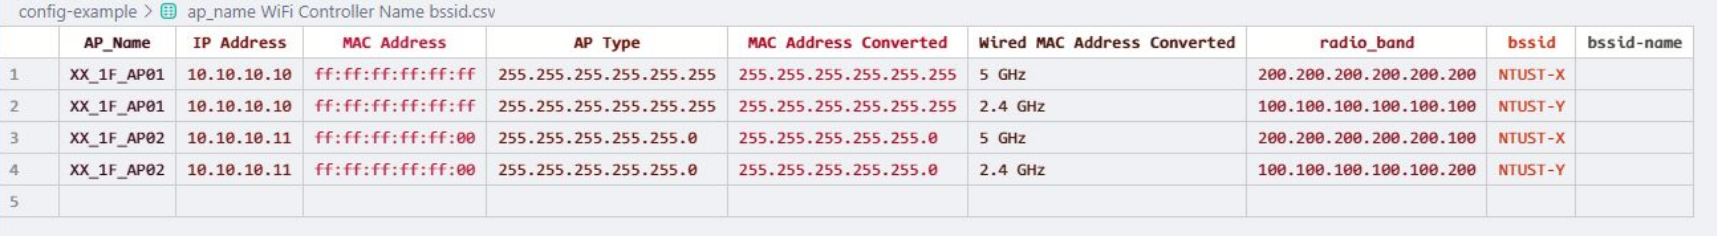
\includegraphics[width=0.8\textwidth]{assets/pics/config_example.png}
    \caption{Template file CSV AP mapping}
    \label{fig:config_example}
\end{figure}

Pada gambar \ref{fig:config_example} ditunjukkan template file CSV yang digunakan untuk memetakan AP Aruba berdasarkan BSSID. File ini berisi informasi penting seperti nama AP, alamat IP, alamat MAC, tipe AP, pita radio, SSID, dan BSSID.

% %-----------------------------------------------------------------------------%
% \subsubsection{Aktivitas Integrasi dan Visualisasi SMO}
% Integrasi dengan SMO melibatkan beberapa kegiatan debugging dan penyempurnaan:
% \begin{itemize}
%     \item Memperbaiki format XML PM agar sesuai dengan ekspektasi \textit{parser} SMO.
%     \item Mengedit label dan melakukan sanitasi data untuk memastikan konsistensi.
%     \item Mengimplementasikan fungsionalitas API tambahan, seperti \texttt{DELETE} untuk menghapus pekerjaan PM yang sudah ada dari \textit{managed element}.
%     \item Mempersiapkan dan menginstal pustaka yang diperlukan di lingkungan server untuk mendukung komunikasi NETCONF.
% \end{itemize}
% Data yang berhasil dikumpulkan dan disimpan di InfluxDB kemudian divisualisasikan menggunakan \textbf{Grafana}, yang memungkinkan pemantauan metrik \textit{real-time} seperti jumlah klien (\texttt{clients}) dari waktu ke waktu.

% \begin{figure}[htbp]
%     \centering
%     % \includegraphics[width=0.8\textwidth]{grafana_dashboard.png}
%     \caption{Dashboard Grafana yang menunjukkan data klien (Slide 10)}
%     \label{fig:grafana_dashboard}
% \end{figure}

%

% \section{Proyek 1: WiFi Adapter untuk Integrasi O-RAN}
% %-----------------------------------------------------------------------------%
% Proyek ini bertujuan untuk membuat komponen perangkat lunak yang dapat mengumpulkan data dari infrastruktur WiFi di dunia nyata dan memformatnya agar sesuai dengan spesifikasi antarmuka O-RAN O1 untuk sistem \textit{Service Management and Orchestration} (SMO).

% \subsection{Pengembangan dan Fungsionalitas}
% Tahap awal pengembangan berfokus pada implementasi \textit{WiFi Adapter} untuk mengirimkan data \textit{Performance Management} (PM) ke SMO. Data ini mencakup metrik penting seperti RSSI dan jumlah klien, yang diformat sebagai laporan berbasis file (JSON/XML) dan dikirim melalui SFTP.

% Untuk mendukung interoperabilitas, arsitektur adapter dirancang secara modular dengan beberapa kelas utama: \textit{Connection, Crawler, Converter, Vault,} dan \textit{Database}. Fokus utama adalah pada implementasi untuk perangkat dari vendor Aruba dan HPE. Skrip Python dikembangkan untuk mengekstrak metadata dari \textit{Access Point} (AP) Aruba dan switch HPE menggunakan protokol SNMP.
% \begin{itemize}
%     \item \textbf{Data AP Aruba yang Dikumpulkan:} Nama host AP (\textit{AP\_Name}), alamat IP manajemen, alamat MAC, model AP (\textit{AP Type}), pita frekuensi radio (\textit{radio\_band}), dan detail SSID/BSSID.
%     \item \textbf{Data Switch HPE yang Dikumpulkan:} Data pemetaan port yang menghubungkan perangkat (AP) ke port switch fisik, termasuk \textit{Port Name}, \textit{Switch Hostname}, dan \textit{PoE Type}.
% \end{itemize}
% Selama pengembangan, penulis melakukan pengujian \textit{crawling} PoE, debugging masalah \textit{crawling} RSSI, menangani pengambilan kredensial dari beberapa database, dan mencocokkan parameter agar sesuai dengan standar O-RAN.

% \subsection{Integrasi dengan SMO}
% Tahap selanjutnya adalah mengintegrasikan data yang dikumpulkan dengan struktur PM di SMO. Kegiatan pada tahap ini meliputi:
% \begin{itemize}
%     \item Memperbaiki kesalahan pada format XML PM agar sesuai dengan ekspektasi SMO.
%     \item Mengedit label dan melakukan sanitasi data.
%     \item Mengimplementasikan fitur seperti penghapusan file PM dan pengaturan tanggal kedaluwarsa file.
%     \item Mempersiapkan integrasi NETCONF dengan menginstal pustaka yang diperlukan di lingkungan server.
% \end{itemize}
% Kegiatan integrasi SMO ini sebagian besar dilakukan pada awal Oktober 2025.

%-----------------------------------------------------------------------------%
\section{Proyek 2: Simulator RSSI Sionna dan Pipeline Lokalisasi}
%-----------------------------------------------------------------------------%
Proyek ini merupakan inti dari penelitian ``Wifi RAN Digital Twin'', yang berfokus pada pembuatan lingkungan kembaran digital untuk analisis propagasi sinyal dan pemodelan lokalisasi.

\subsection{Pengembangan Aplikasi Simulator Sionna}
Penulis mengembangkan aplikasi Python bernama \texttt{RSSI\_App.py} yang menggunakan NVIDIA Sionna untuk menyimulasikan propagasi sinyal dan memperkirakan nilai RSSI. Arsitektur aplikasi, diagram kelas, dan diagram urutan juga dirancang untuk mendokumentasikan sistem. Untuk simulasi, sebuah lingkungan 3D dari denah lantai gedung dibuat menggunakan Blender.

Salah satu bagian penting dari proyek ini adalah kalibrasi parameter. Metode \textit{parameter sweeping} diimplementasikan untuk mengeksplorasi efek dari berbagai parameter, seperti efek material (konduktivitas, permitivitas, koefisien hamburan, dan ketebalan dinding). Metode optimisasi hibrida yang menggabungkan CMA-ES dan Adam (\texttt{06\_hybrid-optimization\_4-params.py}) digunakan untuk menyetel parameter simulasi agar hasilnya cocok dengan data RSSI yang diukur di dunia nyata. Aplikasi ini menghasilkan output berupa \textit{heatmap}, plot, dan dataset sidik jari.

\subsection{Implementasi Pipeline Lokalisasi}
Sebagai bukti konsep (\textit{Proof-of-Concept}), model lokalisasi sederhana dikembangkan menggunakan K-Nearest Neighbors (KNN) dan dataset sederhana. Selain itu, model klasifikasi ruangan juga dibuat.

Pipeline lokalisasi yang lebih lengkap diimplementasikan dengan alur sebagai berikut:
\begin{enumerate}
    \item Dataset sidik jari dihasilkan menggunakan parameter simulasi yang telah dikalibrasi.
    \item Eksperimen lokalisasi KNN dijalankan (\texttt{02\_rssi-knn-for-ap.ipynb}) menggunakan sidik jari yang dihasilkan dan dibandingkan dengan data RSSI AP dari dunia nyata.
    \item Selain itu, penulis juga menjalankan kembali dan memodifikasi eksperimen lokalisasi \textit{Rogue AP} berbasis XGBoost yang sudah ada sebelumnya, dan mengintegrasikan Sionna untuk visualisasi/pemetaan lokasi yang diprediksi.
\end{enumerate}

%-----------------------------------------------------------------------------%
\section{Proyek 3: Layanan Sinkronisasi GitHub ke Trello}
%-----------------------------------------------------------------------------%
Penulis memberikan kontribusi signifikan dalam meningkatkan dan memelihara layanan sinkronisasi dua arah yang dirancang untuk menyelaraskan log harian dan \textit{milestone} antara file Markdown di GitHub dan kartu di Trello.

Pekerjaan berpusat pada debugging, finalisasi, dan refaktorisasi basis kode. Beberapa perbaikan bug kritis yang berhasil diselesaikan antara lain:
\begin{itemize}
    \item \textbf{Efek ``Ping-Pong'':} Masalah yang disebabkan oleh perbedaan stempel waktu kecil yang menyebabkan sinkronisasi berulang tanpa henti.
    \item \textbf{Batas 50 Komentar API Trello:} Diatasi dengan mengimplementasikan paginasi berbasis kursor.
    \item \textbf{Duplikasi Aturan Horizontal:} Memperbaiki kesalahan pemformatan Markdown.
\end{itemize}
Selain perbaikan bug, fitur baru juga dikembangkan, yaitu resolusi konflik antar komentar yang dapat dikonfigurasi. Fitur ini memungkinkan pengguna memilih strategi resolusi, seperti \texttt{more\_recent} (berdasarkan stempel waktu) atau \texttt{more\_characters} (mempertahankan konten yang lebih detail). Penulis juga membuat dokumentasi yang komprehensif (termasuk dokumentasi Sphinx) dan video demo untuk alat ini.

%-----------------------------------------------------------------------------%
\section{Riset, Analisis, dan Aktivitas Pendukung}
%-----------------------------------------------------------------------------%
Selain proyek-proyek utama, penulis juga terlibat dalam berbagai kegiatan penelitian, analisis, dan pendukung.

\subsection{Pengumpulan Data Awal dengan Web Scraping}

Sebelum implementasi \textit{WiFi Adapter} berbasis SNMP, fokus awal adalah mengumpulkan data dari perangkat Ubiquiti Unifi menggunakan \textit{web scraping}. Penulis meneliti berbagai metode pengumpulan data dan memilih Playwright untuk melakukan \textit{scraping} pada dasbor Unifi. Skrip yang dikembangkan mampu menangani login, navigasi, menangkap data AP secara berkala (Nama AP, Alamat IP, Klien, Throughput, dll.), melakukan hashing pada alamat IP/MAC, dan menyimpan data ke format JSON atau mengunggahnya langsung ke InfluxDB.


\subsection{Studi Konsep O-RAN dan Wifi RAN}
Penulis mempelajari standar O-RAN, dengan fokus pada Spesifikasi Antarmuka O1 (WG10). Dari studi ini, tiga fase untuk pengembangan \textit{WiFi Adapter} diformalkan: 1) pengiriman data PM melalui VES/SFTP, 2) konfigurasi melalui NETCONF, dan 3) kontrol penuh SMO sebagai produsen MNS.

\subsection{Analisis Kasus Penggunaan Data WiFi}
Penulis menganalisis berbagai kasus penggunaan data WiFi, termasuk prediksi beban untuk penghematan energi, estimasi propagasi AP menggunakan Sionna, pembuatan profil pergerakan pengguna, deteksi anomali tanpa pengawasan, dan analisis waktu tinggal (\textit{dwell-time}). Analisis data RSSI juga dilakukan, di mana penulis mempelajari konsep dasar elektromagnetik dan analisis deret waktu.

\subsection{Logistik dan Dokumentasi}
Tugas-tugas lain yang dilakukan meliputi:
\begin{itemize}
    \item \textbf{Administrasi/Infrastruktur:} Memperbaiki masalah pada server/PC lab (akses Proxmox, masalah login Ubuntu, mengambil perangkat keras lab, dan menangani penyimpanan penuh pada server InfluxDB).
    \item \textbf{Pengembangan Situs Web Lab:} Mengerjakan perombakan komprehensif situs web BMW Lab menggunakan Google Sites.
    \item \textbf{Dokumentasi Resmi:} Menyusun log KP dan laporan KP menggunakan LaTeX, membuat dan merevisi video testimoni dan penjelasan proyek, serta menyiapkan berbagai slide presentasi.
    \item \textbf{Manajemen Peserta Magang Baru:} Membuat sumber daya pembelajaran, rencana studi, dan tugas untuk peserta magang baru.
\end{itemize}